\PassOptionsToPackage{svgnames}{xcolor}
\documentclass[12pt]{article}



\usepackage[margin=1in]{geometry}  
\usepackage{graphicx}             
\usepackage{amsmath}              
\usepackage{amsfonts}              
\usepackage{framed}               
\usepackage{amssymb}
\usepackage{array}
\usepackage{amsthm}
\usepackage[nottoc]{tocbibind}
\usepackage{bm}
\usepackage[object=vectorian]{pgfornament} 
\colorlet{shadecolor}{lightgray!25}
\newcommand{\sectionline}{%
  \noindent
  \begin{center}
  {\color{DarkViolet}
    \resizebox{0.5\linewidth}{1ex}
    {{%
    {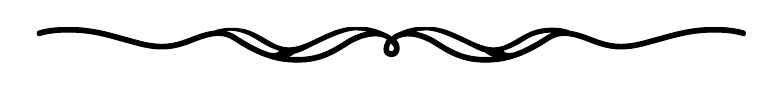
\begin{tikzpicture}
    \node  (C) at (0,0) {};
    \node (D) at (9,0) {};
    \path (C) to [ornament=85] (D);
    \end{tikzpicture}}}}}%
    \end{center}
  }

 \newcommand{\im}{\mathrm{i}}
  \newcommand{\diff}{\mathrm{d}}
\setlength{\parindent}{0cm}
\setlength{\parskip}{0em}
\newcommand{\Lim}[1]{\raisebox{0.5ex}{\scalebox{0.8}{$\displaystyle \lim_{#1}\;$}}}
\newtheorem{definition}{Definition}[section]
\newtheorem{theorem}{Theorem}[section]
\theoremstyle{definition}
\DeclareMathOperator{\arcsec}{arcsec}
\DeclareMathOperator{\arccot}{arccot}
\DeclareMathOperator{\arccsc}{arccsc}
\setcounter{tocdepth}{1}
\begin{document}
\title{Revision notes - MA1102R}
\author{Ma Hongqiang}
\maketitle
\tableofcontents

\clearpage

\section{Limits}
\subsection{Precise Definition of Limits}
\begin{definition}[Limit]
\hfill\\
\normalfont Let $f$ be a function defined on an open interval containing $a$, except possibly at $a$.\\
The \textbf{limit} of $f(x)$ when $x$ approaches $a$, equals $L$ if\\
\textbf{for every} $\epsilon>0$ \textbf{there is} a $\delta_{\epsilon}>0$ such that
\[
|f(x)-L|<\epsilon\;\;\;\;\text{whenever}\;\;\;\;0<|x-a|<\delta_{\epsilon}
\]
\end{definition}
\begin{definition}[Left-hand Limit]
\hfill\\
\normalfont We write $\Lim{x\to a^{-}}f(x)=L$ if\\
\textbf{for every} $\epsilon>0$ \textbf{there is} a $\delta>0$ such that
\[
|f(x)-L|<\epsilon\;\;\;\;\text{whenever}\;\;\;\;0<a-x<\delta
\]
\end{definition}
\begin{definition}[Right-hand Limit]
\hfill\\
\normalfont We write $\Lim{x\to a^{-}}f(x)=L$ if\\
\textbf{for every} $\epsilon>0$ \textbf{there is} a $\delta>0$ such that
\[
|f(x)-L|<\epsilon\;\;\;\;\text{whenever}\;\;\;\;0<x-a<\delta
\]
\end{definition}
\begin{definition}[Infinite Limit]
\hfill\\
\normalfont We write $\Lim{x\to a^{-}}f(x)=\infty$ if
\textbf{for every} $M>0$ \textbf{there is} a $\delta>0$ such that
\[
f(x)>M\;\;\;\;\text{whenever}\;\;\;\;0<|x-a|<\delta
\]
\end{definition}
\begin{definition}[Negative Infinite Limit]
\hfill\\
\normalfont We write $\Lim{x\to a^{-}}f(x)=-\infty$ if
\textbf{for every} $M<0$ \textbf{there is} a $\delta>0$ such that
\[
f(x)<M\;\;\;\;\text{whenever}\;\;\;\;0<|x-a|<\delta
\]
\end{definition}
\subsection{Law of Limits}
\begin{theorem}[Scalar Multiplication Law]
\hfill\\
\normalfont If $\Lim{x\to a}f(x)=L$, then $\Lim{x\to a} (c(f(x)))=cL$, where $c$ is a constant.
\end{theorem}
\begin{theorem}[Sum Law]
\hfill\\
\normalfont If $\Lim{x\to a}f(x)=L$ and $\Lim{x\to a}g(x)=M$, then $\Lim{x\to a}(f(x)+g(x))=L+M$.
\end{theorem}
\begin{theorem}[Product Law]
\hfill\\
\normalfont If $\Lim{x\to a}f(x)=L$ and $\Lim{x\to a}g(x)=M$, then $\Lim{x\to a}f(x)g(x)=LM$.
\end{theorem}
\begin{theorem}[Quotient Law]
\hfill\\
\normalfont If $\Lim{x\to a}f(x)=L$ and $\Lim{x\to a}g(x)=M$, then $\Lim{x\to a}\frac{f(x)}{g(x)}=\frac{L}{M}$ provided that $M\neq 0$.
\end{theorem}
\begin{theorem}
\hfill\\
\normalfont Suppose $f(x)=g(x)$ for all $x$ near $a$, except possibly at $a$.\\
If $\Lim{x\to a}f(x)=L$, then $\Lim{x\to a}g(x)$ exists and equals $L$.
\end{theorem}
\begin{theorem}[Inequality on Limits]
\hfill\\
\normalfont Suppose $f(x)\leq g(x)$ for all $x$ near $a$, except possibly at $a$.\\
If $\Lim{x\to a}f(x)=L$ and $\Lim{x\to a}g(x)=M$, then $L\leq M$.
\end{theorem}
\begin{theorem}[Squeeze Theorem]
\hfill\\
\normalfont Let $f,g,h$ be functions such that $f(x)\leq g(x)\leq h(x)$ for all $x$ near $a$, and $\Lim{x\to a}f(x)=\Lim{x\to a}h(x)=L$\\
Then $\Lim{x\to a}g(x)$ exists and equals $L$.
\end{theorem}
\clearpage
\section{Continuous Functions}
\subsection{Continuity at a Point}
\begin{definition}[Continuity at Point]
\hfill\\
\normalfont A function $f$ is \textbf{continuous at a number} $a$ if
\[
\lim_{x\to a}f(x)=f(a)
\]
\end{definition}
The definition of continuity requires the following:
\begin{enumerate}
\item $f$ is \textbf{defined} at $a$,
\item $\Lim{x\to a}f(x)$ exists,
\item $\Lim{x\to a}f(x)=f(a)$.
\end{enumerate}
\begin{definition}[One-sided continuity]
\hfill\\
\normalfont A function $f$ is said to \textbf{be continuous from the right} at $a$ if
\[
\lim_{x\to a^{+}}f(x)=f(a)
\]
and $f$ is said to \textbf{be continuous from the left} at $a$ if
\[
\lim_{x\to a^{-}}f(x)=f(a)
\]
\end{definition}
\begin{theorem}
\hfill\\
\normalfont $f$ is \textbf{continuous at} $a$ \textit{if and only if} $f$ is \textbf{continuous from the left at }$a$ and \textbf{continuous from the left at} $a$.
\end{theorem}
\subsection{Continuity on an Interval}
\begin{definition}[Continuity on Interval]
\hfill\\
\normalfont $f$ is \textbf{continuous on an interval} if it is \textbf{continuus at every number} in the interval.
\end{definition}
$f$ is continuous on open interval $(a,b)$
\[
\Leftrightarrow f \text{ is continuous at every }x\in(a,b)
\]
$f$ is continuous on closed interval $[a,b]$
\[
\Leftrightarrow \begin{cases}
                  f\text{ is continuous at every }x\in(a,b)\\
                  f\text{ is continuous from the right at }a\\
                  f\text{ is continuous from the left at }b
                \end{cases}
\]
\subsection{Properties of Continuous Function}
Suppose $f$ and $g$ are continuous at $a$, then
\begin{itemize}
\item $cf$ is continuous at $a$,
\item $f+g$ is continuous at $a$,
\item $fg$ is continuous at $a$,
\item $f/g$ is continuous at $a$, provided that $g(a)\neq 0$.
\end{itemize}
\textbf{Polynomials}, \textbf{rational functions}, \textbf{root functions}, \textbf{trigonometric functions} are continuous over domain.
\begin{theorem}[Composite of Continuous Functions]
\hfill\\
\normalfont If $f$ is \textbf{continuous} at $b$ and $\Lim{x\to a}g(x)=b$, then
\[
\lim_{x\to a}f(g(x))=f(b)
\]
Or equivalently,
\[
\lim_{x\to a}f(g(x))=f\left(\Lim{x\to a}g(x)\right)
\]
\end{theorem}
If $g$ is continuous at $a$ and $f$ is continuous at $g(a)$, then the \textbf{composite} $f\circ g$ is continuous at $a$.
\subsubsection{Remarks on substitution}
Suppose $y=g(x)$ such that $\Lim{x\to a}g(x)=b$. If
\begin{enumerate}
\item $f$ is \textbf{continuous} at $b$; \textbf{or}
\item $g(x)\neq b$ for all $x$ near $a$, and $\Lim{y\to b}f(y)$ exists;
\end{enumerate}
Then $\Lim{x\to a}f(g(x))=\Lim{y\to b}f(y)$.\\
In particular, assuming that $\Lim{y\to b}f(y)$ exists, then (2) holds if $g$ is a \textbf{one-to-one} function
\subsection{Intermediate Value Theorem}
\begin{theorem}[Intermediate Value Theorem(Simple)]
\hfill\\
\normalfont Let $f$ be a function \textbf{continuous on} a finite closed interval $[a,b]$.\\
If $f(a)<0$ and $f(b)>0$, or if $f(a)>0$ and $f(b)<0$, then\\
there exists a number $c\in(a,b)$ such that $f(c)=0$.
\end{theorem}
\begin{theorem}[Intermediate Value Theorem]
\hfill\\
\normalfont Let $f$ be a function \textbf{continuous on}  $[a,b]$ with $f(a)\neq f(b)$.\\
Let $N$ be a number between $f(a)$ and $f(b)$, then \textbf{there exists} $c\in(a,b)$ such that $f(c)=N$.
\end{theorem}
\clearpage 
\section{Derivatives}
\begin{definition}[Derivative]
\hfill\\
\normalfont The \textbf{derivative} of a function $f$ at a number $a$ is
\[
f^\prime (a):=\lim_{h\to 0}\frac{f(a+h)-f(a)}{h}
\]
$f$ is differentiable at $a$ if $f^\prime (a)$ exists.\\
$f^\prime (a)$ is the slope of $y=f(x)$ at $x=a$.\\
An equivalent definition is:
\[
f^\prime (a):=\lim_{x\to a}\frac{f(x)-f(a)}{x-a}
\]
\end{definition}
\begin{theorem}[Differentiability implies Continuity]
\hfill\\
\normalfont If $f$ is \textbf{differentiable} at $a$ then $f$ is \textbf{continuous} at $a$.
\end{theorem}
\begin{theorem}[Differentiation Formulas]
\hfill\\
\normalfont
\begin{itemize}
\item $(cf)^\prime=cf^\prime$
\item $(f\pm g)^\prime=f^\prime\pm g^\prime$
\item $(fg)^\prime=f^\prime g + fg^\prime$
\item $\left(\frac{f}{g}\right)^\prime=\frac{f^\prime g -fg^\prime}{g^2}$, if $g(x)\neq 0$.
\end{itemize}
\end{theorem}
\begin{theorem}[Some useful results]
\hfill\\
\normalfont
\begin{itemize}
\item $(x^n)^\prime=nx^{n-1}$ for all $n\in\mathbb{Q}$
\item Lemma A: $\Lim{\theta\to 0}\frac{\sin\theta}{\theta}=1$
\item Lemma B: $\Lim{\theta\to 0}\frac{1-\cos\theta}{\theta}=0$
\item $(\sin x)^\prime = \cos x$
\item $(\cos x)^\prime = -\sin x$
\item $(\tan x)^\prime = \sec^{2}x$
\item $(\cot x)^\prime = -\csc^{2}x$
\item $(\sec x)^\prime = \sec x\tan x$
\item $(\csc x)^\prime = -\csc x\cot x$
\end{itemize}
\end{theorem}
\begin{theorem}[Chain Rule]
\hfill\\
\normalfont Let $f$ and $g$ be differentiable functions.\\
Then $F=f\circ g$ is differentiable and 
\[
F^\prime = (f^\prime \circ g)(g^\prime)
\]
\end{theorem}
\clearpage
\section{Applications of Differentiation}
\begin{definition}[Absolute Maximum and Minimum]
\hfill\\
\normalfont Let $f$ be a function, and $D$ be its domain.\\
$f$ has an \textbf{global} (or \textbf{absolute}) \textbf{maximum} at $c \in D$
\[\Leftrightarrow f(c) \geq f(x) \text{ for all }x \in D.\]
$f$ has an \textbf{global} (or \textbf{absolute}) \textbf{minimum} at $c \in D$
\[\Leftrightarrow f(c) \leq f(x) \text{ for all }x \in D.\]
The \textbf{absolute maximum} and \textbf{absolute minimum} are called the \textbf{(absolute) extreme values}.
\end{definition}
\begin{definition}[Local Maximum and Minimum]
\hfill\\
\normalfont Let $f$ be a function with domain $D$.\\
$f$ has a \textbf{local maximum} at $c \in D$
\[ \Leftrightarrow f(c) \geq f(x)\text{ for all }x \text{ near }c\text{ (i.e., for all }x\text{ in an open interval containing }c)\]
$f$ has a \textbf{local minimum} at $c \in D$
\[\Leftrightarrow f(c) \leq f(x)\text{ for all }x\text{ near }c\text{ (i.e., for all }x\text{ in an open interval containing }c)\]
\end{definition}
\begin{theorem}[Extreme Value Theorem]
\hfill\\
\normalfont If $f$ is \textbf{continuous} on a \textbf{finite closed} interval $[a,b]$, then $f$ attains \textbf{extreme values} on $[a,b]$.\\
Precisely, $f$ attains an
\begin{itemize}
\item \textbf{absolute maximum} value $f(c)$ at some $c\in[a,b]$,
\item \textbf{absolute minimum} value $f(d)$ at some $d\in[a,b]$.
\end{itemize}
\end{theorem}
\begin{theorem}[Finding Extreme Values]
\hfill\\
\normalfont Let $f$ be a continuous function on closed interval $[a, b]$.
\begin{enumerate}
\item Compute the values at \textbf{endpoints}: $f(a)$, $f(b)$.
\item Find \textbf{local max} and \textbf{local min} of $f$ on $(a,b)$.
\item Compare the values obtained above to seek out the \textbf{extreme values}.
\end{enumerate}
\end{theorem}
\begin{theorem}[Fermat's Theorem]
\hfill\\
\normalfont Suppose $f$ has a \textbf{local maximum} or \textbf{local minimum} at $c$.
\[
\text{If }f^\prime (c)\text{ exists, then }f^\prime (c)=0
\]
\end{theorem}
\begin{definition}[Critical Number]
\hfill\\
\normalfont Let $f$ be a function with domain $D$.\\
Then $c \in D$ is called a \textbf{Critical Number} of $f$ if
 $f^\prime (c)$ does not exist, or $f^\prime (c)$ exists and equals $0$.
\end{definition}
\begin{theorem}[Closed Interval Method]
\hfill\\
\normalfont Condition: $f$ is a \textbf{continuous} function on interval $[a, b]$. 
\begin{enumerate}
\item Find the values of $f$ at \textbf{endpoints}: $x = a$, $x = b$,
\item Find the values of $f$ at \textbf{critical numbers} of $f$ in $(a, b)$
\item Compare the values of $f(x)$ evaluated in 1 and 2.
\end{enumerate}
\end{theorem}
\begin{theorem}[Rolle's Theorem]
\hfill\\
\normalfont Condition: $f$ is a function such that
\begin{itemize}
\item $f$ is \textbf{continuous} on $[a,b]$,
\item $f$ is \textbf{differentiable} on $(a,b)$,
\item $f(a)=f(b)$
\end{itemize}
Then there is a number $c\in(a,b)$ such that $f^\prime (c)=0$.
\end{theorem}
\begin{theorem}[Mean Value Theorem]
\hfill\\
\normalfont Condition: $f$ is a function such that
\begin{itemize}
\item $f$ is \textbf{continuous} on $[a,b]$,
\item $f$ is \textbf{differentiable} on $(a,b)$,
\end{itemize}
Then there is a number $c\in(a,b)$ such that
\[
f^\prime (c)=\frac{f(b)-f(a)}{b-a}
\]
\end{theorem}
\begin{theorem}[Cauchy's Mean Value Theorem]
\hfill\\
\normalfont Condition: $f,g$ are functions \textbf{continuous} on $[a,b]$, \textbf{differentiable} on $(a,b)$, and $g^\prime (x)\neq 0$ for any $x\in (a,b)$. \\
Then there exists $c\in (a,b)$ such that
\[
\frac{f^\prime (c)}{g^\prime (c)}=\frac{f(b)-f(a)}{g(b)-g(a)}
\]
\end{theorem}
\begin{theorem}[An application of Mean Value Theorem]
\hfill\\
\normalfont Let $f$ be a function such that
\begin{itemize}
\item $f$ is \textbf{continuous} on $[a,b]$
\item $f^\prime (x)=0$ for any $x\in(a,b)$
\end{itemize}
Then $f$ is \textbf{constant} on $[a,b]$.\\
From this theorem, let $f$ and $g$ be continuous on $[a, b]$.\\
If $f^\prime (x)=g^\prime (x)$ for all $x\in(a,b)$, then $f(x)=g(x)+C$ on $[a,b]$ for a constant $C$.
\end{theorem}
\begin{theorem}[Increasing and Decreasing Test]
\hfill\\
\normalfont Condition: $f$ is \textbf{continuous} on $[a,b]$, \textbf{differentiable} on $(a,b)$.\\
If $f^\prime (x)>0$ for any $x\in(a,b)$, then $f$ is \textbf{increasing} on $[a,b]$.\\
If $f^\prime (x)<0$ for any $x\in(a,b)$, then $f$ is \textbf{decreasing} on $[a,b]$.\\
\end{theorem}
\begin{theorem}[Weak Converse of Increasing Test]
\hfill\\
\normalfont Let $f$ be \textbf{differentiable} on an open interval $I$.
\begin{itemize}
\item $f$ is \textbf{increasing} $\Leftrightarrow f^\prime\geq 0$ on $I$.
\item $f$ is \textbf{decreasing} $\Leftrightarrow f^\prime\leq 0$ on $I$.
\end{itemize}
\end{theorem}
\begin{theorem}[First Derivative Test]
\hfill\\
\normalfont Condition: $f$ is a \textbf{continuous} function, and $c$ is a \textbf{critical number} of $f$. Suppose $f$ is \textbf{differentiable} near $c$, except possibly at $c$.
\begin{itemize}
\item If $f^\prime$ changes from \textbf{positive} to \textbf{negative} at $c$, then $f$ has a \textbf{local maximum} at $c$.
\item If $f^\prime$ changes from \textbf{negative} to \textbf{positive} at $c$, then $f$ has a \textbf{local minimum} at $c$.
\item If $f^\prime$ does not change sign at $c$, then $f$ has \textbf{neither local max/min} at $c$.
\end{itemize}
\end{theorem}
\begin{definition}[Concavity]
\hfill\\
\normalfont The graph of $f$ is \textbf{concave up} on open interval $I$ if $f(x) > f^\prime (y)(x - y) + f(y)$ for any $x \neq y$ in $I$.\\
The graph of $f$ is \textbf{concave down} on open interval $I$ if $f(x) < f^\prime(y)(x - y) + f(y)$ for any $x\neq y$ in $I$.
\end{definition}
\begin{theorem}[Relations of Concavity and $f^\prime$]
\hfill\\
\normalfont Condition: $f$ is \textbf{differentiable} on an open interval $I$.
\begin{itemize}
\item The graph is \textbf{concave up} $\Leftrightarrow f^\prime$ is \textbf{increasing}.
\item The graph is \textbf{concave down} $\Leftrightarrow f^\prime$ is \textbf{decreasing}.
\end{itemize}
\end{theorem}
\begin{theorem}[Concavity Test]
\hfill\\
\normalfont Condition: $f$ is \textbf{twice differentiable} on an open interval $I$.
\begin{itemize}
\item If $f^{\prime\prime} > 0 $ on $I$, by increasing test, $f^\prime$ is increasing, then the graph of $f$ is \textbf{concave up}.
\item If $f^{\prime\prime} < 0 $ on $I$, by decreasing test, $f^\prime$ is decreasing, then the graph of $f$ is \textbf{concave down}.
\end{itemize}
\textbf{Remark}: Concavity, however, only requires $f$ be differentiable.
\end{theorem}
\begin{theorem}[Second Derivative Test]
\hfill\\
\normalfont Condition: $f^{\prime\prime}$ exists at \textbf{critical numbers} and $f^{\prime\prime}$ is non-zero at \textbf{critical numbers}.
\begin{itemize}
\item $f^\prime (c)=0$ and $f^{\prime\prime}(c)>0 \Rightarrow f$ has a \textbf{local minimum} at $c$.
\item $f^\prime (c)=0$ and $f^{\prime\prime}(c)<0 \Rightarrow f$ has a \textbf{local maximum} at $c$.
\end{itemize}
\end{theorem}
\begin{definition}[Inflection Point]
\hfill\\
\normalfont A point $P$ on the curve of $y = f(x)$ is called an \textbf{inflection point} if
\begin{itemize}
\item  $f$ is \textbf{continuous} at $P$, and
\item  the \textbf{concavity} of the curve changes at $P$.
\end{itemize}
\end{definition}
\begin{theorem}[Properties of Inflection Point]
\hfill\\
\normalfont Suppose $f$ has an inflection point at $c$, if $f$ is \textbf{twice differentiable} at $c$, then $f^{\prime\prime}(c)=0$.
\end{theorem}
\begin{theorem}[Taylor's Theorem]
\hfill\\
\normalfont Suppose $f$ is $n+1$ times differentiable, then,
\[
f(x)=f(a)+f^\prime (a)(x-a) +\frac{f^{\prime\prime}(a)}{2}(x-a)^2 +\cdots + \frac{f^{(n)}(a)}{n!} +R_n\]
\[\text{where }R_n=\frac{f^{(n+1)}(c)}{(n+1)!}(x-a)^{n+1}\text{ for a }c\text{ between }x\text{ and }a.
\]
\end{theorem}
\begin{theorem}[l'Hopital's Rule]
\hfill\\
\normalfont Conditions:
\begin{itemize}
\item $\Lim{x\to a} f(x) =\Lim{x\to a}g(x)=0\text{ or }\infty$
\item $f$ and $g$ are \textbf{differentiable} near $a$, except at $a$
\item $g^\prime (x)\neq 0$ near $a$.
\end{itemize}
Then $\Lim{x\to a}\frac{f(x)}{g(x)}=\Lim{x\to a}\frac{f^\prime (x)}{g^\prime (x)}$, provided that the limit on the right hand side exists or equal $\pm\infty$
\end{theorem}
\clearpage
\section{Integrals}
\begin{definition}[Definite Integral]
\hfill\\
\normalfont Condition: $f$ is a \textbf{continuous} function on $[a,b]$.\\
The \textbf{definite integral} of $f$ from $a$ to $b$:
\[
\int_{a}^{b} f(x)\diff x=\Lim{n\to \infty}\sum_{i=1}^{n}f(a+i\frac{b-a}{n})\frac{1}{n}
\]
\end{definition}
\begin{theorem}[Properties of Definite Integral]
\hfill\\
\normalfont
\begin{itemize}
\item $\int_{a}^{b} f(x)\diff x = -\int_{b}^{a} f(x)\diff x $ 
\item $\int_{a}^{b} c\diff x = (b-a)c$
\item $\int_{a}^{b} c f(x)\diff x = c\int_{a}^{b} f(x)\diff x$
\item $\int_{a}^{b} (f(x)+g(x))\diff x = \int_{a}^{b} f(x)\diff x+\int_{a}^{b} g(x)\diff x$
\item $\int_{a}^{c} f(x)\diff x + \int_{c}^{b} f(x)\diff x = \int_{a}^{b} f(x)\diff x$
\item Let $f$ be a continuous function on $[a,b]$,($a<b$). Suppose $f(x)\geq 0$ on $[a,b]$, then $\int_{a}^{b} f(x)\diff x\geq 0$.
\item Let $f$ and $g$ be continuous and $f(x)\geq g(x)$ on $[a,b]$, then $\int_{a}^{b} f(x)\diff x\geq \int_{a}^{b} g(x)\diff x$
\item Let $f$ be continuous and $m\leq f(x)\leq M$ on $[a,b]$. $m(b-a)\leq \int_{a}^{b} f(x)\diff x\leq M(b-a)$
\end{itemize}
\end{theorem}
\begin{theorem}[Fundamental Theorem of Calculus (I)]
\hfill\\
\normalfont Let $f$ be a \textbf{continuous} function on $[a,b]$. Define $g(x) = \int_{a}^{x} f(t)\diff t$. Then
\begin{itemize}
\item $g$ is \textbf{continuous} on $[a,b]$
\item $g$ is \textbf{differentiable} on $(a,b)$, and $g^\prime (x) = f(x)$ on $(a,b)$.
\end{itemize}
\end{theorem}
\begin{theorem}[Fundamental Theorem of Calculus (II)]
\hfill\\
\normalfont Let $f$ be a \textbf{continuous} function on $[a,b]$. If $F$ is \textbf{continuous} on $[a,b]$ and $F^\prime = f$ and $[a,b]$, then
\[
\int_{a}^{b} f(x)\diff x = F(b)-F(a)
\]
\end{theorem}
\begin{theorem}[Substitution Rule]
\hfill\\
\normalfont Let $u=g(x)$ be a differentiable function whose range is an interval. If $f$ is continuous and $g^\prime$ is continuous, then
\[
\int f(g(x))g^\prime (x)\diff x=\int f(u)\diff u
\]
\[
\int^{b}_{a} f(g(x))g^\prime (x)\diff x=\int ^{g(b)}_{g(a)} f(u)\diff u
\]
\end{theorem}
\begin{definition}[Improper Integral]
\hfill\\
\normalfont Let $f$ be \textbf{continuous} on $[a,b)$, and discontinuous at $b$.
\[
\int_{a}^{b} f(x)\diff x  = \Lim{t\to b^-}\int_{a}^{t} f(x)\diff x 
\]
\end{definition}
\begin{theorem}[Properties of Improper Integral]
\hfill\\
\normalfont Suppose $f$ has a discontinuity at $c\in (a,b)$.
\[
\int_{a}^{b} f(x)\diff x =\int_{a}^{c} f(x)\diff x +\int_{c}^{b} f(x)\diff x\text{ if both are convergent} 
\] 
\end{theorem}
\begin{definition}[Improper Integral over Infinite Intervals]
\hfill\\
\normalfont If $\int_{a}^{t} f(x)\diff x$ exists for every $t\geq a$, the improper integral of $f$ from $a$ to $\infty$ is 
\[
\int_{a}^{\infty} f(x)\diff x=\Lim{t\to \infty}\int_{a}^{t} f(x)\diff x  
\] 
\end{definition}
\clearpage
\section{Inverse Functions and Techniques of Integration}
\begin{definition}[One to One Function]
\hfill\\
\normalfont $f$ is said to be \textbf{one-to-one} if
\[
\text{for any }a,b\in D, a\neq b\Rightarrow f(a)\neq f(b)
\]
Or equivalently,
\[
\text{for any }a,b\in D, f(a)=f(b)\Rightarrow a=b
\]
\end{definition}
\begin{definition}[Inverse Function]
\hfill\\
\normalfont Let $f$ be a \textbf{one-to-one} function with domain $A$ and range $B$.\\
Its \textbf{inverse function} $f^{-1}$ is the function with 
\begin{itemize}
\item \textbf{domain} $B$ and \textbf{range} $A$, and
\item $f^{-1}(y)=x\Leftrightarrow y=f(x)$ for any $x\in A, y \in B$.
\end{itemize}
\end{definition}
\begin{theorem}[Calculus of Inverse Function]
\hfill\\
\normalfont Let $f$ be a one-to-one continuous function on an open interval $I$, then the inverse function $f^{-1}$ is also continuous.
\begin{itemize}
\item If $f$ is \textbf{differentiable} at $a\in I$, and $f^\prime (a)\neq 0$,
\item then $f^{-1}$ is \textbf{differentiable} at $b=f(a)$,
\item[] and $(f^{-1})^\prime (b) = \frac{1}{f^\prime(a)}$
\end{itemize}
\end{theorem}
\subsection{Inverse Trigonometric Functions}
\begin{table}[h]
\centering
\begin{tabular}{|c|c|c|}
\hline
Inverse Function&Domain&Range\\\hline
$\arcsin x$&$[-1,1]$&$[-\frac{\pi}{2},\frac{\pi}{2}]$\\\hline
$\arccos x$&$[-1,1]$&$[0,\pi]$\\\hline
$\arctan x$&$\mathbb{R}$&$(-\frac{\pi}{2},\frac{\pi}{2})$\\\hline
$\arccot x$&$\mathbb{R}$&$(0,\pi)$\\\hline
$\arcsec x$&$\mathbb{R}\setminus (-1,1)$&$[0,\frac{\pi}{2})\cup[\pi,\frac{3\pi}{2})$\\\hline
$\arccsc x$&$\mathbb{R}\setminus (-1,1)$&$(0,\frac{\pi}{2}]\cup(\pi,\frac{3\pi}{2}]$\\\hline
\end{tabular}
\end{table}
\subsection{Derivative of Inverse Trigonometric Functions}
\begin{itemize}
\item $\frac{\diff}{\diff x}\arcsin x = \frac{1}{\sqrt{1-x^2}},-1<x<1$
\item $\frac{\diff}{\diff x}\arccos x = \frac{-1}{\sqrt{1-x^2}},-1<x<1$
\item $\frac{\diff}{\diff x}\arctan x = \frac{1}{1+x^2},x\in\mathbb{R}$
\item $\frac{\diff}{\diff x}\arccot x = \frac{-1}{1+x^2},x\in\mathbb{R}$
\item $\frac{\diff}{\diff x}\arcsec x = \frac{1}{x\sqrt{x^2-1}},|x|>1$
\item $\frac{\diff}{\diff x}\arccsc x = \frac{-1}{x\sqrt{x^2-1}},|x|>1$
\item[] And following are the identities.
\item $\arcsin x + \arccos x = \frac{\pi}{2}$
\item $\arctan x + \arccot x = \frac{\pi}{2}$
\item $\arcsec x + \arccsc x =  
										\begin{cases}
											\frac{\pi}{2},\text{  if } x\geq 1\\
											\frac{5\pi}{2},\text{if } x\leq -1\\
											\end{cases}$

\end{itemize}
\subsection{Natural Logarithmic Function}
\begin{definition}[Natural Logarithmic Function($\ln x$)]
\hfill\\
\[
\ln x= \int ^{x}_{1}\frac{1}{t}\diff t
\]
\end{definition}
\begin{theorem}[Properties of Natural Logarithmic Function]
\hfill\\
\normalfont
\begin{itemize}
\item $\ln 1 = 0, \ln e = 1$
\item $\ln x$ is increasing on $\mathbb{R}^+$
\item $\Lim{x\to\infty}\ln x = \infty, \Lim{x\to\infty}\ln x = -\infty$
\item Let $a>0$ and $x>0$. $\ln ax=\ln a +\ln x$
\item Let $x>0$. $\ln x^r = r\ln x$.
\item $\int \frac{1}{x}\diff x = \ln |x| + C$
\end{itemize}
\end{theorem}
\begin{theorem}[Logarithmic Differentiation]
\hfill\\
\normalfont Given $y=f_1(x)f_2(x)\cdots f_n(x)$, we have
\[
\ln|y| = \ln|f_1(x)|+\ln|f_2(x)|+\cdots+ \ln|f_n(x)|
\]
\[
\frac{1}{y}\frac{\diff y}{\diff x} = \frac{f^\prime_1(x)}{f_1(x)}+\cdots+\frac{f^\prime_n(x)}{f_n(x)}
\]
\[
\frac{\diff y}{\diff x} = \left[\frac{f^\prime_1(x)}{f_1(x)}+\cdots+\frac{f^\prime_n(x)}{f_n(x)}\right]f_1(x)f_2(x)\cdots f_n(x)
\]
\end{theorem}
\subsection{Exponential Function}
\begin{definition}[Exponential Function]
\hfill\\
\normalfont Exponential function (exp $x$), is defined as
\[
e^x=\ln ^{-1}(x), \text{ for all }x\in \mathbb{R}
\]
\end{definition}
\begin{theorem}[Properties of Exponential Function]
\begin{itemize}
\item $\Lim{x\to\infty}e^x=\infty, \Lim{x\to-\infty}e^x=0$
\item $\Lim{x\to\infty} \frac{e^{x}}{x^{n}}=\infty, n\in \mathbb{Z}^{+}$
\item $e^x = \sum^{\infty}_{n=0}\frac{x^n}{n!}$
\end{itemize}
\end{theorem}
\begin{definition}[(Generalised) Exponential Function]
\hfill\\
\normalfont For $a>0$ and $x\in \mathbb{R}$, define
\[
a^x=\text{exp}(x\ln a) = e^{x\ln a}\]
\end{definition}
\begin{theorem}[More Properties of Exponential Function]
\hfill\\
\normalfont
\begin{enumerate}
\item $a^u a^v = a^{u+v}$
\item $a^{-u}=\frac{1}{a^u}$
\item $(a^u)^v=a^{uv}$
\item $(a^x)^\prime = a^x \ln a$
\item $\int x^r \diff x = \begin{cases}
								\frac{x^{r+1}}{r+1}+C \text{ if }r\neq -1\\
								\ln|x| +C \text{if }r=-1
								\end{cases}$
\item $e = \Lim{x\to 0}(1+x)^{\frac{1}{x}} = \Lim{y\to\infty}(1+\frac{1}{y})^y$
\end{enumerate}
\end{theorem}
\subsection{Hyperbolic Trigonometric Functions}
\begin{definition}[Hyperbolic Trigonometric Functions]
\hfill\\
\normalfont 
\begin{itemize}
\item $\sinh x = \frac{e^x-e^{-x}}{2}$
\item $\cosh x = \frac{e^x+e^{-x}}{2}$
\item[] Remark:
\item[] $\cosh^2 x -\sinh^2 x = 1$
\item[] $(\sinh x)^\prime = \cosh x, (\cosh x)^\prime = \sinh x$
\item $\tanh x = \frac{\sinh x}{\cosh x}$
\end{itemize}
\end{definition}
\begin{theorem}[Inverse Trigonometric Functions]
\hfill\\
\normalfont Let $y = \sinh^{-1} x$. $\frac{\diff}{\diff x}\sinh^{-1} x =\frac{\diff y}{\diff x} = \frac{1}{\frac{\diff x}{\diff y}} = \frac{1}{\cosh y} = \frac{1}{\sqrt{1+x^2}}$\\
Hence, $\sinh^{-1} x = \ln(x+\sqrt{1+x^2}), x\in\mathbb{R}$.\\
Similarly,\\
 $\cosh^{-1} x = \ln(x+\sqrt{x^2-1}), x\geq 1$; \\
 $\tanh^{-1} x = \frac{1}{2}\ln\left(\frac{1+x}{1-x}\right),-1<x<1$
\end{theorem}
\subsection{More Techniques on Integration}
\begin{theorem}[Substitution Rule(2nd version)]
\hfill\\
\normalfont Let $f$ be a continuous function, and $x=g(t)$ be a differentiable function. If $g^\prime$ is continuous, then
\[
\int f(x)\diff x = \int f(g(t))g^\prime(t)\diff t
\]
\end{theorem}
\subsubsection{Useful Substituents}
\begin{table}[h]
\centering
\begin{tabular}{|c|c|}
\hline
Scenario& Substituent\\\hline
$\frac{1}{x(1+x^4)}$&$x=\frac{1}{t}$\\\hline
$1+x^2$&$x=\tan t$\\\hline
$\sqrt{1-x^2}$&$x=\sin t$\\\hline
$\sqrt{x^2-1}$&$x=\sec t$\\\hline
$\sin x,\cos x,\cdots$ &$t=\tan\frac{x}{2}$\\\hline
$\frac{f(x)}{g(x)}$, $f,g$ polynomial&Partial fraction\\\hline
\end{tabular}
\end{table}
\begin{theorem}[Integration by Parts]
\hfill\\
\normalfont
\[
\int u\diff v = uv - \int v\diff u
\]
\end{theorem}
\clearpage
\section{Application of Integral}
\begin{theorem}[Finding Net Area]
\hfill\\
\normalfont Let $f$ be a \textbf{continuous} function on $[a,b]$. Then the \textbf{net area} under $y=f(x)$ from $a$ to $b$ is
\[
A=\int^b_a f(x)\diff x
\]
\end{theorem}
\begin{theorem}[Finding Volume (Washer Method)]
\hfill\\
\normalfont Suppose the solid is obtained by rotating the region between the curve $y=f(x)$ and the $x$-axis from $a$ to $b$ about the $x$-axis.
\[
V=\int^b_a \pi(f(x))^2 \diff x
\]
\end{theorem}
\begin{theorem}[Finding Volume (Cylindrical Shell Method)]
\hfill\\
\normalfont Let $f$ be a continuous function such that $f(x)\geq 0$ for all $x\in[a,b]$ where $0\leq a<b$. Then the volume of the solid obtained by rotating the region between the curve $y=f(x)$ and the $x$-axis from $a$ to $b$ about the $y$-axis is
\[
V=\int^b_a 2\pi xf(x)\diff x
\]
\end{theorem}
\begin{theorem}[Finding Arc Length]
\hfill\\
\normalfont The \textbf{arc length} of smooth curve $y=f(x)$ from $x=a$ to $x=b$ is
\[
L=\int^b_a\sqrt{1+(f^\prime(x))^2}\diff x
\]
\end{theorem}
\begin{theorem}[Finding Surface Area of Revolution]
\hfill\\
\normalfont Let $f$ be a smooth function such that $f(x)\geq 0$ on $[a,b]$. Then the area of the surface obtained by rotating the curve $y=f(x), a\leq x\leq b$ about the $x$-axis is
\[
A=\int^b_a 2\pi f(x)\sqrt{1+(f^\prime(x))^2}\diff x
\]
\end{theorem}
\clearpage
\section{Ordinary Differential Equations}
\subsection{Simplest Ordinary Differential Equations}
\[
\frac{\diff y}{\diff x}=f(x)\Rightarrow y=\int f(x)\diff x + C
\]
\[
\frac{\diff y}{\diff x}=g(y)\Rightarrow \frac{\diff x}{\diff y}=\frac{1}{g(y)}\Rightarrow x=\int\frac{1}{g(y)}\diff y
\]
\subsection{Seperation of Variables}
Consider $\frac{\diff y}{\diff x} = f(x)g(y)$.\\
In \textbf{differential forms}, $\frac{1}{g(y)}\diff y = f(x)\diff x$\\
\[
\int \frac{1}{g(y)}\diff y =\int f(x)\diff x
\]
Remark: Try substitute $z=\frac{y}{x}$ when encountering homogeneous equations of degree zero.
\subsection{First Order Linear Equations}
\begin{definition}[First Order Linear Equations]
\hfill\\
\normalfont First order linear equations are in the form
\[
\frac{\diff y}{\diff x}+p(x)y=q(x)
\]
\end{definition}
\begin{theorem}[Solving First Order Linear Equations]
\hfill\\
\normalfont Consider $\frac{\diff y}{\diff x}+p(x)y=q(x)$.
\begin{itemize}
\item Evaluate $P(x) = \int p(x)\diff x$
\item Let $v(x) = e^{P(x)}$
\item $y =\frac{1}{v(x)}\int v(x)q(x)\diff x$
\end{itemize}
\end{theorem}
\begin{theorem}[Bernoulli's Equation]
\hfill\\
\normalfont Consider $\frac{\diff y}{\diff x}+p(x)y=q(x)y^n$.\\
Substitute $z=y^{1-n}$. We have $\frac{\diff z}{\diff x}+(1-n)p(x)z=(1-n)q(x)$.
\end{theorem}
\clearpage

\end{document}